\documentclass[12pt,twoside,a4paper]{report}
\usepackage{etex}
% Select encoding of your inputs.
\usepackage[utf8]{inputenc}

% Make latex understand and use the typographic
% rules of the language used in the document.
\usepackage[english]{babel}

% Use the vector font Latin Modern which is going
% to be the default font in latex in the future.
\usepackage{lmodern}
% Use vector arrows in mathmode
\usepackage{esvect}

% Choose the font encoding
\usepackage[T1]{fontenc}

% load a colour package
\usepackage[table]{xcolor}
\definecolor{aaublue}{RGB}{33,26,82}% dark blue

% The standard graphics inclusion package
\definecolor{white}{RGB}{255,255,255} % define color white
\usepackage{graphicx}

% Set up how figure and table captions are displayed
\usepackage{caption}
\captionsetup{%
  font=footnotesize,% set font size to footnotesize
  labelfont=bf % bold label (e.g., Figure 3.2) font
}

% Enable row combination in tables
\usepackage{multirow}

% Make space between table lines and text
\renewcommand{\arraystretch}{1.5}

% Make the standard latex tables look so much better
\usepackage{array,booktabs}

% Enable the use of frames around, e.g., theorems
% The framed package is used in the example environment
\usepackage{framed}
\usepackage{colortbl}
\usepackage{longtable}

\usepackage{textcomp}

%%%%%%%%%%%%%%%%%%%%%%%%%%%%%%%%%%%%%%%%%%%%%%%%
% Mathematics
%%%%%%%%%%%%%%%%%%%%%%%%%%%%%%%%%%%%%%%%%%%%%%%%
% Defines new environments such as equation,
% align and split 
\usepackage{amsmath}
\usepackage{relsize}
% Adds new math symbols
\usepackage{amssymb}
% Use theorems in your document
% The ntheorem package is also used for the example environment
% When using thmmarks, amsmath must be an option as well. Otherwise \eqref doesn't work anymore.
\usepackage[framed,amsmath,thmmarks]{ntheorem}

%%%%%%%%%%%%%%%%%%%%%%%%%%%%%%%%%%%%%%%%%%%%%%%%
% Page Layout
%%%%%%%%%%%%%%%%%%%%%%%%%%%%%%%%%%%%%%%%%%%%%%%%
% Change margins, papersize, etc of the document
\usepackage[
  left=25mm,% left margin on an odd page %tidligere 25mm for baade right og left
  right=25mm,% right margin on an odd page
  top=35mm,
  ]{geometry}
  
% Modify how \chapter, \section, etc. look
% The titlesec package is very configureable
\usepackage{titlesec}
\makeatletter
\def\ttl@mkchap@i#1#2#3#4#5#6#7{%
    \ttl@assign\@tempskipa#3\relax\beforetitleunit
    \vspace{\@tempskipa}%<<<<<< REMOVE THE * AFTER \vspace
    \global\@afterindenttrue
    \ifcase#5 \global\@afterindentfalse\fi
    \ttl@assign\@tempskipb#4\relax\aftertitleunit
    \ttl@topmode{\@tempskipb}{%
        \ttl@select{#6}{#1}{#2}{#7}}%
    \ttl@finmarks  % Outside the box!
    \@ifundefined{ttlp@#6}{}{\ttlp@write{#6}}}
\makeatother

\titlespacing{\chapter}{0pt}{0pt}{10pt}
\titlespacing{\section}{0pt}{0pt}{-5pt}
\titlespacing{\subsection}{0pt}{8pt}{-5pt}
\titlespacing{\subsubsection}{0pt}{6pt}{-10pt}

\titleformat*{\section}{\normalfont\Large\bfseries}%\color{aaublue}}
\titleformat*{\subsection}{\normalfont\large\bfseries}%\color{aaublue}}
\titleformat*{\subsubsection}{\normalfont\normalsize\bfseries}%\color{aaublue}}
%\titleformat*{\paragraph}{\normalfont\normalsize\bfseries\color{aaublue}}
%\titleformat*{\subparagraph}{\normalfont\normalsize\bfseries\color{aaublue}}

%Formatting chapter headers. Predefined styles that can be used as option to the package: Sonny, Lenny, Glenn, Conny, Rejne, Bjarne, PetersLenny and Bjornstrup

%\usepackage[Sonny]{fncychap}

\usepackage{titlesec, blindtext, color}
%\definecolor{gray75}{gray}{0.75}
\newcommand{\hsp}{\hspace{20pt}}
\titleformat{\chapter}[hang]{\Huge\bfseries}{\thechapter\hsp{|}\hsp}{0pt}{\Huge\bfseries}


% Change the headers and footers
\usepackage{fancyhdr}
\setlength{\headheight}{15pt}
\pagestyle{fancy}
\fancyhf{} %delete everything
\renewcommand{\headrulewidth}{0pt} %remove the horizontal line in the header
\fancyhead[RO,LE]{\small\nouppercase\leftmark} %even page - chapter title

\fancyhead[LO]{}
\fancyhead[RE]{} 
\fancyhead[CE]{}
\fancyhead[CO]{}

\fancyfoot[RE,LO]{\thepage}
\fancyfoot[LE,RO]{B205} %page number on all pages
\fancyfoot[CE,CO]{}



% change first page of all chapters header and footer to fancy style
\makeatletter
\let\ps@plain\ps@fancy
\makeatother

% Do not stretch the content of a page. Instead,
% insert white space at the bottom of the page
\raggedbottom

% Enable arithmetics with length. Useful when typesetting the layout.
\usepackage{calc}

%%%%%%%%%%%%%%%%%%%%%%%%%%%%%%%%%%%%%%%%%%%%%%%%
% Bibliography
%%%%%%%%%%%%%%%%%%%%%%%%%%%%%%%%%%%%%%%%%%%%%%%%
% Add the \citep{key} command which display a
% reference as [author, year]

\usepackage[square]{natbib}

%\usepackage{natbib}
% Appearance of the bibliography
\bibliographystyle{setup/apalike}

%%%%%%%%%%%%%%%%%%%%%%%%%%%%%%%%%%%%%%%%%%%%%%%%
% Misc
%%%%%%%%%%%%%%%%%%%%%%%%%%%%%%%%%%%%%%%%%%%%%%%%

% Add bibliography and index to the table of
% contents
\usepackage[nottoc, notlof, notlot]{tocbibind}
\usepackage{tocloft}
% Add the command \pageref{LastPage} which refers to the
% page number of the last page
\setlength{\cftbeforetoctitleskip}{0 cm}

\usepackage[
  %disable, %turn off todonotes
  colorinlistoftodos, %enable a coloured square in the list of todos
  %inline,
  textwidth=20mm, %set the width of the todonotes
  textsize=scriptsize, %size of the text in the todonotes
  ]{todonotes}
\setlength{\marginparwidth}{2cm}
\newcommand{\todocheck}[1]{\todo[color=green!40, author=Check]{#1}}
\newcommand{\todojens}[1]{\todo[color=red!40, author=Jens, inline]{#1}}
%Command for inserting green todo notes as Ole's corrections.
%\renewcommand{\todo}[1]{\todo[noline]{#1}}  
    
\usepackage{wrapfig}
\usepackage{amssymb}
\usepackage{pifont}
% Enables figures with text wrapped tightly around it 

%%% Table of contents %%%%%  
\setcounter{tocdepth}{1}

\renewcommand{\cftpartpresnum}{Part~}
\let\cftoldpartfont\cftpartfont
\renewcommand{\cftpartfont}{\cftoldpartfont\cftpartpresnum}

%%%%%%%%%%%%%%%%%%%%%%%%%%%%%%%%%%%%%%%%%%%%%%%%
% Hyperlinks
%%%%%%%%%%%%%%%%%%%%%%%%%%%%%%%%%%%%%%%%%%%%%%%%

% Enable hyperlinks and insert info into the pdf
% file. Hypperref should be loaded as one of the 
% last packages
\usepackage{nameref}
\usepackage{hyperref}
\hypersetup{%
	%pdfpagelabels=true,%
	plainpages=false,%
	pdfauthor={Author(s)},%
	pdftitle={Title},%
	pdfsubject={Subject},%
	bookmarksnumbered=true,%
	colorlinks,%
	citecolor=black,%
	filecolor=black,%
	linkcolor=black,% you should probably change this to black before printing
	urlcolor=black,%
	pdfstartview=FitH%
}
\urlstyle{same}
% remove all indentations
\setlength\parindent{0pt}
\parskip 5mm
\usepackage{verbatim}


\definecolor{Gra}{RGB}{230,230,230}

%creates a nice-looking C#-text
\newcommand{\CC}{C\nolinebreak\hspace{-.05em}\raisebox{.3ex}{\scriptsize\text \#} }

%enables multi column lists
\usepackage{multicol}

%enables code-examples
\usepackage{listings}



%%%%%%%%%%%%%%%%%%%%%%%%%%%%%%%%%%%%%%%%%%%%%%%%
% Define colors
%%%%%%%%%%%%%%%%%%%%%%%%%%%%%%%%%%%%%%%%%%%%%%%%
\definecolor{coolblue}{RGB}{32,95,128}
\definecolor{mygreen}{rgb}{0,0.6,0}
\definecolor{mygray}{rgb}{0.5,0.5,0.5}
\definecolor{mymauve}{rgb}{0.58,0,0.82}
\usepackage{textcomp}
\definecolor{listinggray}{gray}{0.9}
\definecolor{lbcolor}{rgb}{0.9,0.9,0.9}
\definecolor{tikzblue}{RGB}{65,144,179}




%%%%%%%%%%%%%%%%%%%%%%%%%%%%%%%%%%%%%%%%%%%%%%%%
% Listing
%%%%%%%%%%%%%%%%%%%%%%%%%%%%%%%%%%%%%%%%%%%%%%%%

\usepackage{xcolor}
\colorlet{keyword}{blue!90!black!100}
\colorlet{keyword2}{red!40!blue!85}
\colorlet{comment}{green!60!black!100}
\definecolor{backcolour}{rgb}{0,0,0}
%\usepackage{beramono}% monospaced font with bold variant
\definecolor{backcolourlst}{rgb}{0.97,0.97,0.96}
%\definecolor{backcolourlst}{rgb}{1,0.75,0.80}

\lstset{
%  backgroundcolor=\color{white},   % choose the background color; you must add \usepackage{color} or \usepackage{xcolor}
%  basicstyle=\footnotesize,        % the size of the fonts that are used for the code
%  breakatwhitespace=false,         % sets if automatic breaks should only happen at whitespace
%  breaklines=true,                 % sets automatic line breaking
%  captionpos=t,                    % sets the caption-position to bottom
%  commentstyle=\color{mygreen},    % comment style
%  deletekeywords={...},            % if you want to delete keywords from the given language
%  escapeinside={\%*}{*)},          % if you want to add LaTeX within your code
%  extendedchars=true,              % lets you use non-ASCII characters; for 8-bits encodings only, does not work with UTF-8
%  frame=single,                    % adds a frame around the code
%  keepspaces=true,                 % keeps spaces in text, useful for keeping indentation of code (possibly needs columns=flexible)
%  keywordstyle=\color{blue},       % keyword style
%  language=C++,                 % the language of the code
%  morekeywords={*,...},            % if you want to add more keywords to the set
%  numbers=left,                    % where to put the line-numbers; possible values are (none, left, right)
%  numbersep=5pt,                   % how far the line-numbers are from the code
%  numberstyle=\tiny\color{mygray}, % the style that is used for the line-numbers
%  rulecolor=\color{black},         % if not set, the frame-color may be changed on line-breaks within not-black text (e.g. comments (green here))
%  showspaces=false,                % show spaces everywhere adding particular underscores; it overrides 'showstringspaces'
%  showstringspaces=false,          % underline spaces within strings only
%  showtabs=false,                  % show tabs within strings adding particular underscores
%  stepnumber=1,                    % the step between two line-numbers. If it's 1, each line will be numbered
%  stringstyle=\color{mymauve},     % string literal style
%  tabsize=2,                       % sets default tabsize to 2 spaces
%  title=\lstname                   % show the filename of files included with \lstinputlisting; also try caption instead of title
	backgroundcolor=\color{lbcolor},
	tabsize=4,
	rulecolor=\color{black},
	language=C,
  	basicstyle   = \linespread{1.2} \ttfamily \scriptsize,
  	keywordstyle = \color{keyword}\bfseries,	
  	commentstyle = \color{comment}\bfseries,
  	numbers=left,                   
	numberstyle=\scriptsize,      
	stepnumber=1,                   
	numbersep=8pt,                  
	backgroundcolor=\color{white},  
	showspaces=false,               
	showstringspaces=false,         
	showtabs=false,                 
	backgroundcolor=\color{backcolourlst},
	%frame=single,
	frame=single,                   
	captionpos=b,           
	breaklines=true,        
	breakatwhitespace=false,    
	escapeinside={\%*}{*)}
}
\lstset{
	emph={uint8_t, int8_t, uint16_t, int16_t, uint32_t, int32_t,}, emphstyle={\color{keyword}\bfseries},
    emph={[2]ISR, TCE1, CNT, TCC1, TCD1_OVF_vect},emphstyle={[2]\color{keyword2}\bfseries}%
}



\usepackage{float}
\usepackage{caption}
\usepackage[font=footnotesize,  labelfont=bf] {subcaption}
\usepackage{siunitx}
\sisetup{decimalsymbol=comma}
\sisetup{detect-weight}

\usepackage{enumitem}
%\usepackage[citestyle=authoryear,natbib=true]{biblatex}

% Figures - TIKZ
\usepackage{tikz}
\usepackage[americanresistors,americaninductors,americancurrents, americanvoltages]{circuitikz}


% Wall of text logo

\newcommand{\walloftextalert}[0]{\includegraphics[width=\textwidth]{walloftext.png}}



% URL break fix nede i bibfil

\def\UrlBreaks{\do\/\do-}


\usepackage{pdfpages}

\definecolor{blockcolor}{RGB}{131,187,253}

\tikzstyle{blockbig} = [draw, fill=blockcolor, rectangle, 
    minimum height=3em, minimum width=6em]
\tikzstyle{block} = [draw, fill=blockcolor, rectangle, 
    minimum height=2em, minimum width=2em]
    
\tikzstyle{blockbigclear} = [draw, fill=white, rectangle, 
    minimum height=3em, minimum width=6em]
\tikzstyle{blockclear} = [draw, fill=white, rectangle, 
    minimum height=2em, minimum width=2em]
    
\tikzstyle{sum} = [draw, fill=blockcolor, circle, node distance=1.5cm, minimum size=0.6cm]
\tikzstyle{sumclear} = [draw, fill=white, circle, node distance=1.5cm, minimum size=0.6cm]
\tikzstyle{input} = [coordinate]
\tikzstyle{output} = [coordinate]
\tikzstyle{pinstyle} = [pin edge={to-,thin,black}]

%% Centering columns of custom width
\newcolumntype{P}[1]{>{\centering\arraybackslash}p{#1}}
\newcolumntype{M}[1]{>{\centering\arraybackslash}m{#1}}

\usepackage{empheq}
\newcommand*\widefbox[1]{\fbox{\hspace{2em}#1\hspace{2em}}}


\usepackage{pgfplots}
\pgfplotsset{filter discard warning = true, unbounded coords=discard}
\pgfplotsset{compat = newest}





\usepackage{lastpage}
\usepackage{epstopdf}
\usepackage{graphicx} %Matlab figures
%\usepackage[table]{xcolor}
\setlength{\headheight}{21pt}
\hfuzz=\maxdimen
\tolerance=10000
\hbadness=10000
%
\usepackage{siunitx}% package inclusion and set up of the document
%Creates the aau titlepage
\newcommand{\aautitlepage}[3]{%
  {
    %set up various length
    \ifx\titlepageleftcolumnwidth\undefined
      \newlength{\titlepageleftcolumnwidth}
      \newlength{\titlepagerightcolumnwidth}
    \fi
    \setlength{\titlepageleftcolumnwidth}{0.5\textwidth-\tabcolsep}
    \setlength{\titlepagerightcolumnwidth}{\textwidth-2\tabcolsep-\titlepageleftcolumnwidth}
    %create title page
    \thispagestyle{empty}
    \noindent%
    \begin{tabular}{@{}ll@{}}
      \parbox{\titlepageleftcolumnwidth}{
        \iflanguage{danish}{%
          
\includegraphics[width=\titlepageleftcolumnwidth]{setup/aau_logo_da.pdf}
        }{%
          
\includegraphics[width=\titlepageleftcolumnwidth]{setup/aau_logo_en.pdf}
        }
      } &
      \parbox{\titlepagerightcolumnwidth}{\raggedleft\sf\small
        #2
      }\bigskip\\
       #1 &
      \parbox[t]{\titlepagerightcolumnwidth}{%
      \textbf{Abstract:}\smallskip\par
        \fbox{\parbox{\titlepagerightcolumnwidth-2\fboxsep-2\fboxrule}{%
          #3
        }}
      }\\
    \end{tabular}
    \vfill
    \vspace{-0.5cm}
    \iflanguage{danish}{%
      \noindent{\footnotesize\emph{Rapportens indhold er frit tilgængeligt, men offentliggørelse (med kildeangivelse) må kun ske efter aftale med forfatterne.}}
    }{%
      \noindent{\footnotesize\emph{The content of this report is freely available, but publication (with reference) may only be pursued due to agreement with the author.}}
    }
    \clearpage
  }
}

%Create english project info
\newcommand{\englishprojectinfo}[8]{%
  \parbox[t]{\titlepageleftcolumnwidth}{
    \textbf{Title:}\\ #1\bigskip\par
    \textbf{Theme:}\\ #2\bigskip\par
    \textbf{Project Period:}\\ #3\bigskip\par
    \textbf{Project Group:}\\ #4\bigskip\par
    \textbf{Participant(s):}\\ #5\bigskip\par
    \textbf{Supervisor(s):}\\ #6\bigskip\par
    \textbf{Copies:} #7\bigskip\par
    \textbf{Page Numbers:} Fucking mange!\bigskip\par
    \textbf{Date of Completion:}\\ #8
  }
}

%Create danish project info
\newcommand{\danishprojectinfo}[9]{%
  \parbox[t]{\titlepageleftcolumnwidth}{
    \textbf{Title:}\\ #1\bigskip\par
    \textbf{Theme:}\\ #2\bigskip\par
    \textbf{Project Period:}\\ #3\bigskip\par
    \textbf{Project Group:}\\ #4\bigskip\par
    \textbf{Participants:}\\ #5\bigskip\par
    \textbf{Supervisor:}\\ #6\bigskip\par
    \textbf{Co-supervisor:}\\ #7\bigskip\par
    \textbf{Copies:} #8\bigskip\par
    \textbf{Page Numbers:} 144\bigskip\par
    \textbf{Date of Completion:}\\ #9
  }
}

%Nice-looking reference to other chapters
\newcommand{\chapref}[1]{Chapter \ref{#1}: \nameref{#1}}
\newcommand{\secref}[1]{Section \ref{#1}: \nameref{#1}}
\newcommand{\figref}[1]{\emph{Figure: \ref{#1}}}
\newcommand{\appref}[1]{Appendix \ref{#1}}
\newcommand{\tabref}[1]{\emph{Table: \ref{#1}}}
\newcommand{\coderef}[1]{\emph{Listings: \ref{#1}}}
%\renewcommand{\eqref}[1]{\emph{Equation: (\ref{#1})}}

\newcommand{\iic}[0]{I²C }

%%%%%%%%%%%%%%%%%%%%%%%%%%%%%%%%%%%%%%%%%%%%%%%%
% An example environment
%%%%%%%%%%%%%%%%%%%%%%%%%%%%%%%%%%%%%%%%%%%%%%%%
\theoremheaderfont{\normalfont\bfseries}
\theorembodyfont{\normalfont}
\theoremstyle{break}
\def\theoremframecommand{{\color{aaublue!50}\vrule width 5pt \hspace{5pt}}}
\newshadedtheorem{exa}{Example}[chapter]
\newenvironment{example}[1]{%
		\begin{exa}[#1]
}{%
		\end{exa}
}

\makeatletter
\newcommand{\ChapterOutsidePart}{%
   \def\toclevel@chapter{-1}\def\toclevel@section{0}\def\toclevel@subsection{1}}
\newcommand{\ChapterInsidePart}{%
   \def\toclevel@chapter{0}\def\toclevel@section{1}\def\toclevel@subsection{2}}
\makeatother

\usepackage{bookmark}

\usepackage{mathtools}
\DeclarePairedDelimiter{\ceil}{\lceil}{\rceil}

%\newenvironment{where}{Where:\\}{\\}

\newcommand{\nomunit}[1]{\renewcommand{\nomentryend}{\hspace*{\fill}#1}}
% \usepackage{array} is required
% \usepackage{array} is required

\newcommand{\new}[3]{\begin{tabular}{p{10pt} p{40pt} p{230pt} l} 
&{#1} & {#2} & {$\left[\text{#3}\right]$}
\end{tabular} \vspace{3pt} \nomenclature{#1}{#2}{#3}{}}

\newcommand{\newpar}{\par \vspace{0.4cm}}



\newenvironment{where}{\hspace{6mm}Where:\\}{}
\newcommand{\va}[3]{\begin{tabular}{p{40pt} p{50pt} p{250pt} l} 
&{#1} & {#2} & {$\left[\text{#3}\right]$}
\end{tabular}}


% easy differential operators
\newcommand*\diff{\mathop{}\!\mathrm{d}}
\newcommand*\Diff[1]{\mathop{}\!\mathrm{d^#1}}
% my new macros
%\usepackage{glossaries}

%\newacronym{<label>}{<abbrv>}{<full>}

\newacronym{AAU}{AAU}{Aalborg University}
\newacronym{AIS}{AIS}{automatic identification system}
\newacronym{EPS}{EPS}{electronic power system}
\newacronym{COM}{COM}{communication}
\newacronym{CSP}{CSP}{cubesat space protocol}
\newacronym{ADCS}{ADCS}{attitude determination and control system}
\newacronym{LOG}{LOG}{system log}
\newacronym{FP}{FP}{flight planner}
\newacronym{PCB}{PCB}{printed circuit board}
\newacronym{CAN}{CAN}{controlled area network}
\newacronym{SPI}{SPI}{serial peripheral interface bus}
\newacronym{I2C}{I$^2$C}{inter-integrated circuit}
\newacronym{RTR}{RTR}{remote transmission request}
\newacronym{DLC}{DLC}{data length code}	
\newacronym{CRC}{CRC}{cyclic redundancy check}
\newacronym{ACK}{ACK}{acknowledge}
\newacronym{MSB}{MSB}{most significant bit}
\newacronym{LSB}{LSB}{least significant bit}
\newacronym{REC}{REC}{receive error count}
\newacronym{TEC}{TEC}{transmit error count}
\newacronym{TCP}{TCP/IP}{transmission control protocol/internet protocol}
\newacronym{UDP}{UDP}{user datagram protocol}
\newacronym{RDP}{RDP}{reliable data protovol}
\newacronym{FOV}{FOV}{field of view}
\newacronym{CMOS}{CMOS}{complementary metal-oxide-semiconductor}
\newacronym{CCD}{CCD}{charge-coupled device}
\newacronym{ADC}{ADC}{analog to digital converter}
\newacronym{DAC}{DAC}{digital to analog converter}
\newacronym{BMP}{BMP}{bitmap}
\newacronym{JPEG}{JPEG}{joint photographic experts group}
\newacronym{DCT}{DCT}{discrete cosine transform}
\newacronym{RAM}{RAM}{random access memory}
\newacronym{FPGA}{FPGA}{field programmable gate array}
\newacronym{TIFF}{TIFF}{tagged image file format}
\newacronym{MIPI}{MIPI}{mobile industry processor interface}
\newacronym{RF}{RF}{radio frequency}
\newacronym{CSI}{CSI}{camera serial interface}
\newacronym{PHY}{PHY}{physical layer}
\newacronym{DPHY}{D-PHY}{physical layer type D}
\newacronym{CSI2}{CSI-2}{camera serial interface 2}
\newacronym{LP}{LP}{low power}
\newacronym{HS}{HS}{high state}
\newacronym{DDR}{DDR}{double data rate}
\newacronym{UART}{UART}{universal asynchronous receive/transmitter}
\newacronym{MOSI}{MOSI}{master out slave in}
\newacronym{MISO}{MISO}{master in slave out}
\newacronym{SCK}{SCK}{serial clock}
\newacronym{CS}{CS}{chip select}
\newacronym{TWI}{TWI}{two-wire interface}
\newacronym{SCL}{SCL}{serial clock}
\newacronym{SDA}{SDA}{serial data}
\newacronym{MCU}{MCU}{microcontroller unit}
\newacronym{SRAM}{SRAM}{Static random access memory}
\newacronym{DRAM}{DRAM}{Dynamic random access memory}
\newacronym{SDRAM}{SDRAM}{Synchronous Dynamic random access memory}
\newacronym{FIFO}{FIFO}{First in first out queue}
\newacronym{DDRSDRAM}{DDR SDRAM}{Double Data Rate Synchronous Dynamic random access memory}
\newacronym{SCCB}{SCCB}{serial camera control bus}
\newacronym{CCI}{CCI}{camera control interface}
\newacronym{SD}{SD}{secure digital}
\newacronym{SDHC}{SDHC}{secure digital high capacity}
\newacronym{.csv}{CSV}{Comma Separated Values}
\newacronym{SDK}{SDK}{Software Development Kit}
\newacronym{RTOS}{RTOS}{Real Time Operating System}
\newacronym{CPU}{CPU}{Central Processing Unit}
\newacronym{ISR}{ISR}{Interrupt Service Routine}
\newacronym{IDE}{IDE}{Integrated Development Environment}
\newacronym{HAL}{HAL}{Hardware Abstraction Layer}
\newacronym{RC}{RC}{Remote Controller}

% acronymer der ikke er skrevet op
%PC
%RAW
%YCbCr
%DC
%AC
%RS.232
%RGB \newacronym{RGB}{RGB}{red, green, blue}




 % glossaries stuff
\usepackage{lastpage}
\usepackage{epstopdf}
\usepackage{graphicx} %Matlab figures
%\usepackage[table]{xcolor}
\setlength{\headheight}{21pt}
\hfuzz=\maxdimen
\tolerance=10000
\hbadness=10000
%
\usepackage{siunitx}

%\makeglossaries
\defcitealias{ITU-R}{ITU-R P.676-10}

\defcitealias{401}{CCSDS, 1993}
\defcitealias{SFCG-4-3R3}{SFCC, 1998}
\defcitealias{ITU5}{ITU, 2009}
\defcitealias{ITU3}{ITU, 1997}
\defcitealias{AMSAT}{AMSAT, 1994}
\defcitealias{AMSATIARU}{IARU, 2015}
\defcitealias{monopolVSdipol}{NCJRS, 2016}
\defcitealias{LNA}{AMTL, 2007}
\defcitealias{ARRLPowerLimit}{ARRL, 2016}
\defcitealias{ModulationSpace}{CCSDS, 2009}
\graphicspath{{./figures/}}


\hypersetup{pdfinfo={
Title={Communication Link for a Cubesat}
}}


\begin{document}
%% prærapport %%
\setlength\cftaftertoctitleskip{2pt}
\setlength\cftafterloftitleskip{6pt}
\setlength\cftafterlottitleskip{6pt}
\captionsetup{belowskip=-1.5em}


\selectlanguage{english}
\title{Design of SDR}

\pagestyle{empty} %disable headers and footers
\pagenumbering{roman} %use roman page numbering in the frontmatter I II...
\fancyfoot[RE,LO]{16gr651} %page number on all pages
\fancyfoot[LE,RO]{\thepage}
\fancyhead[LE,LO,RE,RO]{}
%\fancyhead[RO,LE]{\includegraphics[height=16pt]{logo_only.pdf}}
%% indledende formalia %%

%\listoftodos
%\includepdf[pages={1}]{forside.pdf}
\newgeometry{left = 0 cm, right = 0 cm, bottom=1cm}
%\pdfbookmark[0]{Forside}{label:forside}%
\begin{titlepage}
  \addtolength{\hoffset}{0.5\evensidemargin-0.5\oddsidemargin} %set equal margins on the frontpage - remove this line if you want default margins
  \noindent%
  \centering
  \begin{tabular}{@{}p{0.8\textwidth}@{}}
    \toprule[2pt]
    \midrule
    \vspace{0.2cm}
    \begin{center}
    \fontsize{32}{10}\selectfont{\textbf{
      Communication Link for a Cubesat % insert your title here
    }}
    \end{center}
    \begin{center}
      \LARGE{
      An SDR approach
      }
    \end{center}
    \vspace{0.2cm}\\
    \midrule
    \toprule[2pt]
  \end{tabular}  
  
  \centering

   %\vspace{0.55 cm}
\begin{figure}[H]
\centering
%\includegraphics[width=0.95\paperwidth]{figures/forside-cropped.pdf}
%\label{fig:forside}
\end{figure}
%\vfill
%  \vspace{-0.35 cm}
%  \begin{center}
%    {\large
%      P5 project report %Insert document type (e.g., Project Report)
%    }\\
%    \vspace{0.2cm}
%    {\Large
%      Group 514%Insert your group name or real names here
%    }
%  \end{center}
%  \begin{center}
%  Aalborg University\\
%  Electronic Engineering \& IT\\
%  Frederiks Bajersvej 7\\
%  DK-9220 Aalborg
%  \end{center}
\end{titlepage}

\clearpage
\restoregeometry

\pagestyle{fancy}
%{\small
\strut\vfill % push the content to the bottom of the page
\noindent Copyright \copyright{} Aalborg University 2015\par
\vspace{0.2cm}

\noindent This report is compiled in \LaTeX, originally developed by Leslie Lamport, based on Donald Knuth's \TeX. The main text is written in \emph{Computer Modern} pt 11, designed by Donald Knuth. 
%The document is compiled via the website \url{www.overleaf.com}, an online collaborative based \LaTeX-editor with instant preview, which enables multiple persons to edit the document simultaneously.
Flowcharts and diagrams are made using Microsoft Visio, Inkscape and Tikz, a \TeX package for generating graphics. 
\clearpage

\newgeometry{left = 2.5 cm, right = 2.5 cm, bottom=2.5cm}
%\newgeometry{bottom=2.5cm}
%%pagestyle{fancy} %enable headers and footers again

\begin{comment}
\pdfbookmark[0]{Danish title page}{label:titlepage_en}
\aautitlepage{%
  \englishprojectinfo{
    Project Title %title
  }{%
    Analoge kredsløb og systemer %theme
  }{%
    P3: 2. September 2014 - 17. December 2014 %project period
  }{%
    14gr313 % project group
  }{%
    %list of group members
    Amalie Vistoft Petersen\\
    Mikkel Krogh Simonsen\\
    Rasmus Gundorff Sæderup\\
    Simon Bjerre Krogh\\
    Thomas Kær Juel Jørgensen\\
    Thomas 'Godlike' Rasmussen
  }{%
    %list of supervisors
    Tom S. Pedersen

  }{%
    9 % number of printed copies
  }{%
    \today % date of completion
  }%
}{%department and address
  \textbf{Institut for Elektroniske Systemer}\\
  Fredrik Bajers Vej 7\\
  DK-9220 Aalborg Ø\\
  }{% the abstract
  Here is the abstract
}

\cleardoublepage

\end{comment}

\selectlanguage{english}
\pdfbookmark[0]{Titelblad}{label:titelblad}
\aautitlepage{%
  \danishprojectinfo{
    Communication Link for a cubesat\\ - an SDR approach%title
  }{%
    BSc Project (Communication Systems)  %theme
  }{%
    6. Semester %project period
  }{%
    16gr651 % project group
  }{%
    %list of group members
    Amalie Vistoft Petersen\\
    Rasmus Gundorff Sæderup\\
    Thomas Kær Juel Jørgensen
  }{%
    %list of supervisors
    Troels Bundgaard Sørensen
    }{
    Gilberto Berardinelli
    }{%
    3 % number of printed copies
  }
  {%
    \today % date of completion
  }%
}{%department and address
  \textrm{\textbf{Institute of Electronic Systems  }\\
  Fredrik Bajers Vej 7\\
  DK-9220 Aalborg Ø\\}
 }{
In this project, a communication link between a cubesat and a ground station is designed. This includes an investigation of available frequencies as well as performance characteristics of different antenna- and modulation types. From the investigation, it is chosen to use a 10.5 GHz link with a patch antenna and to use both OQPSK as well as 8-PSK modulation. A link budget is constructed, showing an SNR of 2.8 dB at the receiver, yielding a feasible bitrate of 1.3 Mbps in LEO (1000 km) and 900 bps in lunar orbit (384000 km). This link is simulated in MATLAB showing a plausible bit-error rate (BER) of $0.0251 \pm 0.5 \cdot 10^{-4}$  for the lunar link, and $0.0235 \pm 0.5 \cdot 10^{-4}$ for the LEO link, without forward error coding (FEC). Based on this, an Software Defined Radio (SDR) prototype is implemented on two USRP's using LabVIEW. The prototype has various reconfigurable parameters including modulation type, bitrate and carrier frequency.
Synchronization issues are seen at low SNRs, and the BER is up to 18.5 times bigger than what the simulation shows. 
%The prototype is tested and 4/8 requirements set is fulfilled leaving the strictest performance requirements unfulfilled. 
The end result is a reconfigurable SDR that can transmit and decode data using OQPSK and 8-PSK with a bitrate of up to 500 kbps, with a BER of 0.0239 (without FEC) at an SNR of 5 to 6 dB.
}
\restoregeometry

%\restoregeometry

\pdfbookmark[0]{Indholdsfortegnelse}{label:Indhold}
%\tableofcontents

%\printglossary[title=List of Terms,toctitle=Terms and abbreviations,type=\acronymtype]

%\glsaddall
%\printglossary
%\printglossary[type=\acronymtype]


\cleardoublepage

%\chapter*{Preface}\label{ch:forord}%\addcontentsline{toc}{chapter}{Forord}

This bachelor project in Communication Systems has been carried out during the spring of 2016, by a group of three students from Electronics and IT at Aalborg University.

The project regards the development of a communication link between a satellite in space and a ground station, as well as  the development of a prototype implementation of a software defined radio to be used in the link.
%This report and the prototype described in the following is made by a group of three students on sixth semester "Electronics and IT" at Aalborg University.

A general knowledge of electronic engineering and more specifically communication systems is needed to read the report.  

References to sources are of the APA-style, i.e. of the type [\emph{source name/author's surname, year, optional page number}]. Sources are listed in a bibliography at the end of the report, and PDFs, datasheets etc. can be found in the attached ZIP-file. Figures without a source are made by the project group.% Appendices are listed after the bibliography.

This report is organized in three parts. The first part is a technical analysis that goes in depth with antennas, a link budget of the communication link between a satellite and a ground station at AAU, different suitable modulation types and, finally, a requirements for a prototype of the radio to be used in the communication link is established. \\ In part two, the theory, simulation and implementation of the prototype is described. \\ Part three contains the test of the prototype related to the requirements set up for it in part 1. %Finally, part four contains descriptions of how two created antennas was made and descriptions of three test setups utilized in project and their related results.

Special thanks should be addressed to PhD student Dereje Assefa and associate professor John Hansen for helping with the USRP's and LabVIEW. A thanks to assistant engineer Kristian Bank for helping with tests of the antennas in Starlab and for the great help regarding setting up and borrowing measurement equipment. Furthermore, a thanks goes to associate professors Flemming Bjerre Frederiksen and Carles Navarro Manchón for giving a helping hand in finding reading material.

\vspace{0.5\baselineskip}\hfill Aalborg University, \today
\vfill

%% underskrifts afsnit %%

\vspace{1.5\baselineskip}
\begin{minipage}[b]{0.45\textwidth}
 \centering
 \rule{\textwidth}{0.45pt}\\
  Amalie Vistoft Petersen\\
 {\footnotesize apet13@student.aau.dk}
\end{minipage}
\vspace{1.5\baselineskip}
\hfill
\begin{minipage}[b]{0.45\textwidth}
 \centering
 \rule{\textwidth}{0.45pt}\\
  Rasmus Gundorff Sæderup\\
 {\footnotesize rsader13@student.aau.dk}
\end{minipage}

\noindent\makebox[\textwidth][c]{%
\begin{minipage}[b]{0.45\textwidth}
 \centering
 \rule{\textwidth}{0.5pt}
   Thomas Kær Juel Jørgensen\\
 {\footnotesize tkjj13@student.aau.dk}
\end{minipage}}
}
\chapter{Fresnel Zones}


Fresnel zone \citep{Fres1} \citep{Fres2} calculations gives a mean to calculate on how to avoid the interference from the strongest radio signals that are not direct line signal, this can be caused by reflections of obstacles, these reflected signals will have a different phase and when added with the direct line signal, may cause power loss. There are an infinite amount of Fresnel zones, and all will impact the direct line signal.  %Where these Fresnel zones are created, where there exists and infinite amount of them.   %and will make the reflected signals to be out of phase. 

%the impact of out of phase signals caused by reflections of obstacles, on the signal as whole from the transmitter to the receiver.

%are used to calculate the reflections and diffraction loss between an transmitter and a receiver. 
In terms of a radio signal travelling from a transmitter to a receiver it can travel through different paths. It can travel directly without any reflection. %which is the most ideal%. 
Or it could reflect of the ground and thereby carry on to the receiver, or it could be reflected by a hill, and carry on to the receiver. %which is not desirable, but in some circumstances inevitable. 
These reflections can cause a signal loss from the transmitter to the receiver. The receiver does not differentiate between the reflected and the direct line signals, and therefore it will consider both the reflected and the direct line signal as the intended signal \citep{Fres2}. It is important to note that the reflection it self will create an change in phase up to $180^{\circ}$, the lower the incidence angle the closer to $180^{\circ}$.  %So therefore when calculating the Fresnel zones it will take into consideration the reflections and diffraction loss, and will 
\\
\\
If these signals reflect of an obstacle and are out of phase with the direct line signals, they may end up having phase cancellation effect which could end up minimizing the power of the signals. For example two identical radio signals out of phase will cancel each other out and therefore no signal will be received, by the receiver. So therefore when calculating Fresnel zones it must be taken into consideration which out of phase signals from reflections have the most effect on the direct line signal, and make sure that it does not lose a lot of power. 
\\
\\
There are an infinite amount of Fresnel zones, but the most important Fresnel zone is the first one. This is due to that the strongest signals are the ones that are closets to the direct line signal %which travels without any reflections and will have the same power through the path, 
and they always lie in the first Fresnel Zone.  
Which also means that the second, third and so on Fresnel zones are further and further from the Direct signal and obstacles in these will have a lesser impact \citep{introRF}. This can be seen on the following Figure, which is illustrated with 2 Fresnel zones, Fresnel zone 1 and 2:
\begin{figure}[H]
\centering
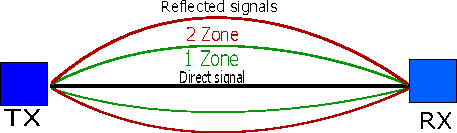
\includegraphics[width=0.6\textwidth]{fresnel_ill_1.pdf}
\caption{Illustration of the First and Second Fresnel zone, along with the Direct signal travelling from the Transmitter TX to the Receiver RX}
\label{dijdk}
\end{figure}

As it can be seen the first Fresnel zone is closets to the direct signal and will have the strongest cancelling effect, if not taken into consideration. It has the least amount of delay in the reflected signal of the first Fresnel zone as it travels least from the transmitter to the receiver. Inside the first Fresnel zone phase delay due to increase in path distance of the reflected wave are $0^\circ$-$90^\circ$, when remembering the phase change done by the reflection itself that means the signal is $180^\circ$-$270^\circ$ out of phase in total. When the reflected signal then interfere with the direct signal destructive interference occur. In terms of the second Fresnel zone, it creates longer phase delay, in total between $270^\circ$ to $450^\circ$ out of phase. This become constructive interference. The phase cancelling effect in even numbered Fresnel zones are good while odd numbered zones are bad. A rule of thumb in terms of the first Fresnel zone is that \textit{$60\%$ of the first Fresnel zone must be cleared of any obstacles}, as this reduces the destructive interference significantly \citep{introRF}\citep{Fres2}. 
\\
\\


\textbf{Fresnel zone 1}
\\
\\
As mentioned $60\%$ of the first Fresnel zone must be cleared of objects, an illustration of this can be seen on the following Figure:
\begin{figure}[H]
\centering
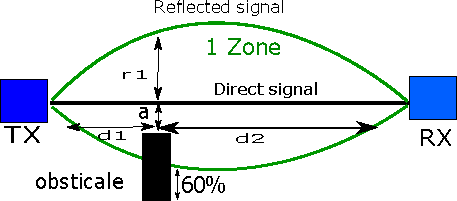
\includegraphics[width=0.6\textwidth]{fresnel_ill_obs.pdf}
\caption{Illustration of the First Fresnel zone cleared $60\%$, with an building representing the obstacle}
\label{dijdk1}
\end{figure}


The obstacle on the Figure above could illustrate a building where $d_{1}$ is the distance from the transmitter $TX$ to the building while $d_{2}$ is the distance from the receiver $RX$ to the building. The radius of the first Fresnel zone is $r_1$. The distance from the direct signal to the obstacle is $a$. 
With this in mind the rule of thumb states that $a > 0.6\cdot r_1$. 


%The obstacle on the Figure above could illustrate a building where $d_{1}$ is the distance from the transmitter $TX$ to the building while $d_{2}$ is the distance from the receiver $RX$ to the building. While $a$ is the center line of sight, which means that there is a obstacle free direct view to the receiver, for the signal to travel. So the building must not be closer than $60\%$ of the measured $r1$ which is the radius of the first Fresnel zone from the center line of sight $a$, to fulfil the requirement of $60\%$ clearance, in the first Fresnel zone. Which in other words means that there must be $60\%$ line of sight, according to the radius of the first Fresnel zone, which represents the impact of the reflected signal ,to travel with the direct signal. %Where the $60\%$ is calculated according to the radius of the first Fresnel zone.

 %where from the center point to the receiver $RX$ shall represent the $60\%$. 

%So $c$ is $r1 \cdot 0.6$



\textbf{Fresnel Zone calculations}

The general equation for calculating the Fresnel zone radius at any point a in between the endpoints is given as \citep{introRF}:

\begin{equation}
F_{n} = \sqrt{\frac{n \lambda d_{1} d_{2}}{d_{1}+d_{2}}}
\label{fres:eq1}
\end{equation}

\begin{where}
\va{$F_{n}$}{The $n^{th}$ Fresnel Zone radius}{m}
\va{$d_{1}$}{The distance of $a$ from TX}{m}
\va{$d_{2}$}{The distance of $a$ from RX}{m}
\va{$\lambda$}{The wavelength of the signal}{m}
\end{where}

A conservative calculation of the $60\%$ rule of thumb is to use the maximum radius of the first Fresnel zone to calculate maximum obstacle heights. %With the maximum radius of the first Fresnel zone and the obstacle height, the maximum obstacle height can be calculated, with respect to $60\%$ clearance. %so that the Transmitter and the Receiver can have LOS, and the first Fresnel zone will be $60\%$ cleared. 


The wavelength $\lambda$ can be expressed as:

\begin{equation}
\lambda = \frac{c}{f}
\label{fres:eq2}
\end{equation}

\begin{where}
\va{$c$}{The speed of light in a vacuum}{3$\cdot$$10^{8}$$ms^{-1}$}
\va{$f$}{Signal frequency}{$Hz$}
\end{where}




%While mostly the interest is the maximum radius of the Fresnel zone 


The maximum radius is found at the point where $d_{1} = d_{2}$. Then by using this as well as setting $n=1$ as it is the first Fresnel zone. An expression for the maximum radius can be found and if \autoref{fres:eq2} is inserted into \autoref{fres:eq1} that yields:


\begin{equation}
r = 8.67 \cdot \sqrt{\frac{D}{f}}
\label{fres:eq3}
\end{equation}

\begin{where}
\va{$D$}{Total distance = $d_{1} + d_{2}$}{km}
\va{$f$}{Signal frequency}{GHz}
\end{where}

As an example to calculate the clearance radius of the first Fresnel zone of two antennas operating 5.5 GHz, with a distance $D$ of 500m. The 60$\%$ clearance radius $a$ is given as:

\begin{equation}
a = 0.60\cdot8.67 \cdot \sqrt{\frac{0.50}{5.5}} = 1.57 m
\label{fres:eq_ex}
\end{equation}

Then by subtracting the antenna height form $a$, the maximum obstacle height with respect to the 60$\%$ clearance can be calculated. So if the the antenna height is 10m, then by subtracting 10m-1.57m we get 8.43 m, which is the maximum obstacle height.  %So to compare with the Figure illustrated with the obstacle \ref{dijdk}, the 10m is the height of the TX and RX where the antennas placed. While the the 60$\%$ clear Fresnel zone maximum radius $r$ is calculated to be 2.02 m. So
%\newpage
%\textbf{Earth curvature}



%http://www.4gon.co.uk/solutions/technical_fresnel_zones.php

%http://radiomobile.pe1mew.nl/?Calculations:Propagation_calculation:Fresnel_zones

%http://www.zytrax.com/tech/wireless/fresnel.htm

%https://s.campbellsci.com/documents/au/technical-papers/line-of-sight-obstruction.pdf

%must lie in the direct line, 

%which is always in the first Fresnel zone. 

%In order to get the maximum signal strength, the effect of the out of phase signals must be minimised.         




%%An illustration of Fresnel zones can be seen on the following Figure:
 




%Fresnel zone radius describes this reflection in relation to the overall path of the signal, which means the whole path from the transmitter to the receiver is taken into account, with the reflections. A reflection can happen anywhere in the path between the transmitter and the receiver.
%\\
%\\
%When a signal is reflected two things can happen:

%\begin{itemize}
%\item The phase of the signal reverses and the signal changes in phase by $180\deg$
%\item As the signal is being reflected and thereby not going in a direct line, it will travel further. Therefore the signal is shifted further in phase, by the difference in path length 
%\label{fres}
%\end{itemize} 
%\chapter{Large Scale Fading}
\label{larg_fad}

Large scale fading \citep{large_scale_fade} \citep{large_scale_fade2} is a result of signal attenuation due to signal propagation over large objects caused by shadowing through surroundings like buildings,hills,trees, streets etc. and losing power. Shadowing is caused by blockage of large objects, where new waves get created as a result of the obstacle. %as there is not pure line of sight.
 And over the whole path it represents the average signal attenuation. An illustration of Shadowing can be seen on the following Figure:
 
\begin{figure}[H]
\centering
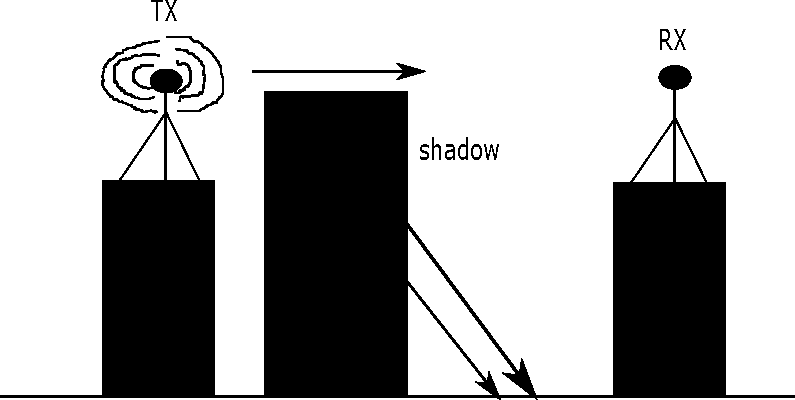
\includegraphics[width=0.6\textwidth]{shadow_ill.pdf}
\caption{Illustration of shadowing caused by an building in between the sender and the receiver}
\label{large_scale_shadow}
\end{figure}

 The path when working with large scale fading is of distances several hundred wavelengths or more. The wavelengths of course depends on the frequency. So when working with Bluetooth or Wi-Fi where the frequency is 2.4 [GHz]. 
%100 wavelengths is 12 [m]. 
Then given the equation for the wavelength:

\begin{equation}
\lambda = \frac{c}{f} = 12 [cm] 
\end{equation}

This gives us one wavelength, this means that for 100 wavelengths this shall be 12[m], which is then considered large scale fading. %In the free space case %with LOS conditions meaning no shadowing, and the receiver and transmitter can see each other with nothing blocking in between, 
%the attenuation of the signal due to distance follows the inverse square law given as:

%\begin{equation}
%\text{Average Signal Attenuation} = \frac{1}{d^{2}} 
%\label{inverse_square_law}
%\end{equation}  

%So the larger the distance from the transmitter to the receiver, the larger the signal attenuation will be. 
%\\
%\\
%In the case of effects caused by trees, buildings etc. The average signal attenuation cannot be characterized as the inverse square law given in \ref{inverse_square_law}, which only holds for free space. The effects of buildings, trees etc. are called shadows, which are waves that are caused by a building or something that is in the way, which creates new waves.
%when there is not pure LOS, meaning that a building or something is in the way, which creates new waves.
%\\
%\\
When taking shadowing into the equation a Lognormal Distribution is used to model the power variation, caused by the effects of shadowing \citep{large_scale_fade3}. The power level in dB is distributed as a Gaussian random variable. The power level in dB at a distance $d$ is given by the following equation:

\begin{equation}
P_{dB}(d) = \overline{P}_{dB}(d)+ \sigma_{dB}X = \overline{P}_{dB}(d_{0}) + 10n\log_{10}(\frac{d}{d_{0}})+ \sigma_{dB}X
\label{power_level}
\end{equation}     

Where $\sigma_{dB}$ is the standard deviation, and $X$ is a standard random variable. It shall be noted that knowledge of $\overline{P}_{dB}(d_{0})$ is required. $\overline{P}_{dB}(d_{0})$ is the path-loss at a distance $d_{0}$. 

A table for $\sigma_{dB}$ values can be seen on the following table:

\begin{figure}[H]
\centering
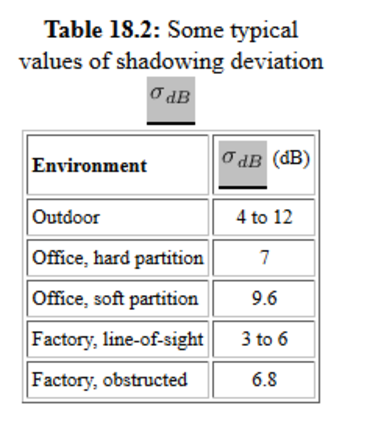
\includegraphics[width=0.3\textwidth]{standard_devi_largescale.pdf}
\caption{Table over the the standard deviation $\sigma_{dB}$ \citep{large_scale_fade3} }
\label{large_scale_shadow_stan_dev_val}
\end{figure}

Where $n$ is path loss exponent, where typical values of $n$ is given in the following table:

\begin{figure}[H]
\centering
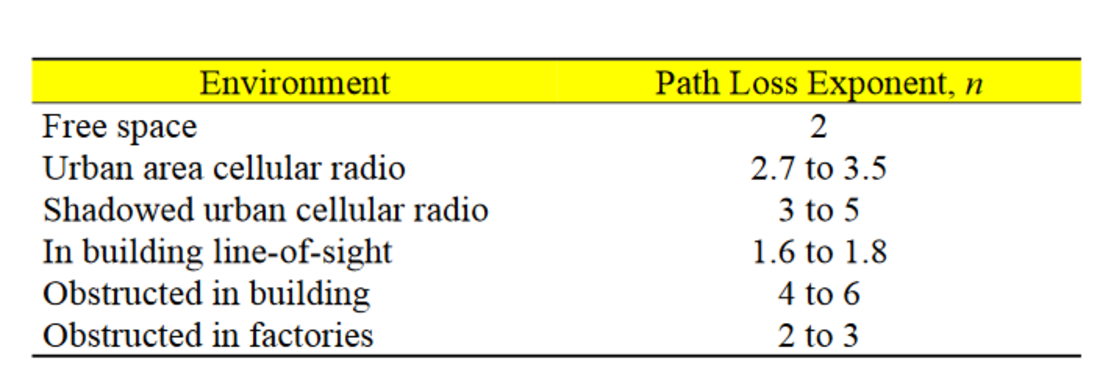
\includegraphics[width=0.6\textwidth]{pathloss_exp_n.pdf}
\caption{Table over the Path loss exponent $n$ \citep{large_scale_fade3} }
\label{large_scale_shadow_pathloss_expo_n}
\end{figure}

%, as the signal will be reflected of buildings.      %In the case of NLOS, which means that the receiver and the transmitter cannot see each other. 

%when working with long distances ()
\chapter{Link Budget}

\begin{figure}[H]
\centering
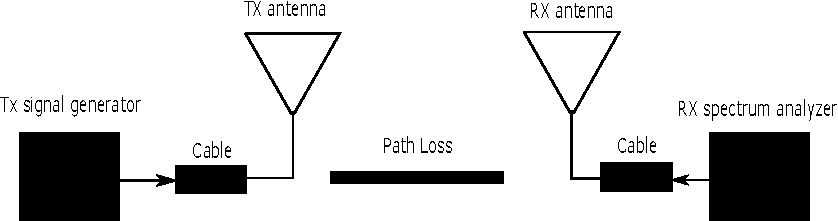
\includegraphics[width=0.7\textwidth]{link_budget_illu.pdf}
\caption{Link budget illustration}
\label{dijdkkfkf}
\end{figure}


%As seen on the Figure above an important aspect for the link 





%A Link budget, takes into account all the losses and gains from the transmitter antenna to the receiver antenna. 
A link budget is calculated to find the received power for the whole system, based on the transmission power, antenna gains, system loss and path loss.

%A Link budget is calculated to take into account the attenuation of the transmitted signal due to propagation, which depends on the circumstances like reflections, free-space loss ,buildings etc. other factors included are cable loss, antenna gains, polarization loss. %which depends if the transmitter antenna and the receiver antenna a pointing directly at each other, if not some loss will occur  etc. 
Such a calculation is given as:

\begin{equation}
P_{r} = \frac{P_{t}G_{t}G_{r}}{L_{p}L_{sys}}
\label{link_calc}
\end{equation}

\begin{where}
\va{$P_{r}$}{Power Received}{W}
\va{$P_{t}$}{Power transmitted}{W}
\va{$G_{t}$}{Transmitter antenna gain}{1}
\va{$L_{p}$}{Path Loss}{1}
\va{$L_{sys}$}{system loss(polarization losses, other losses)}{1}
\va{$G_{r}$}{Receiver antenna gain}{1}
\end{where}
\newpage
\section{Polarization loss factor (PLF)}
Polarization loss \citep{PLF} plays a factor in the link budget calculation. There is linear polarization and circular polarization. For linear polarization the antenna can be turned horizontal and vertical direction this is illustrated in the following Figure:

\begin{figure}[H]
\centering
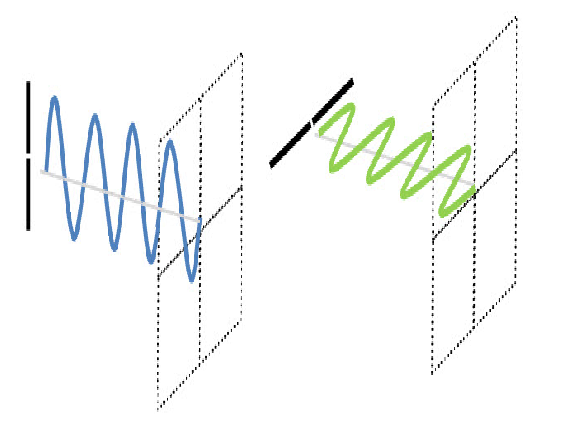
\includegraphics[width=0.4\textwidth]{polariz_ver_hor_lin.pdf}
\caption{Linear horizontal and vertical polarization \citep{plf_illu}}
\label{fig:pol_ver_hor}
\end{figure} 

The PLF for linear polarized antennas can be calculated by the equations given on the following Figure depending on the angle of the the antennas, an illustration of the PLF for max, non and signal loss with dependence on an angle:

\begin{figure}[H]
\centering
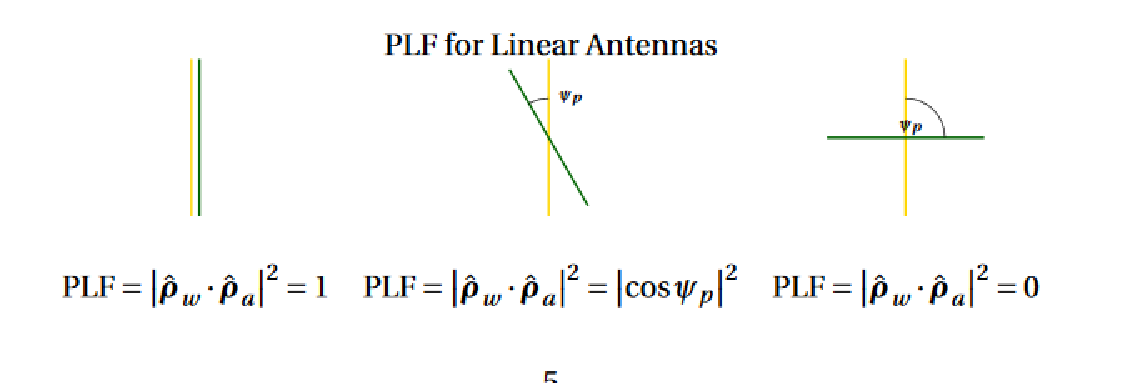
\includegraphics[width=0.6\textwidth]{plf.pdf}
\caption{Minimum, PLF loss depending on the angle and maximum  \citep{plf_illu}}
\label{fig:lin_plf}
\end{figure} 

As it can be seen if the two antennas are pointing directly at each other with the same polarization there will be no PLF. While if one antenna is vertically polarized and the other is horizontally polarized, then no power will be transferred. While there will be some power loss if the two antennas are not $100\%$ aligned, meaning there is an polarization miss match ,there will be some power loss depending on the angle.

\subsection{PLF loss calculated}

For the measurements conducted the PLF factor is calculated with an angle $\psi$ of 5$^{\circ}$, as a margin for the two antennas alignment, this gives the following PLF loss factor:

\begin{equation}
cos(\psi)^{2} = cos(5)^2 = 0.9962
\end{equation}

Then to get it in dB:

\begin{equation}
10 \cdot log(0.9962) = -0.0381dB
\end{equation}



%the angle of the antennas as they are not pointing directly at each other is around  5$^{\circ}$


\section{Cable Loss}
As a part of the link budget cable loss is also included. The cable loss is depended on the length of the cable, where the longer the cable the more cable loss there will be as the signal will lose strength travelling through the cable. Where for each cable it is indicated in the data sheet how much power is lost per meter at different frequencies, this is different for each type of cable. 


\subsection{Calculated cable loss}
Two different types of cables were used these are:

\begin{itemize}
\item rg223/u 
\item SUCOFLEX$\_$104
\end{itemize}

The length for the  rg223/u \citep{rg} cable is of 1m, while for the SUCOFLEX$\_$104 cable \citep{sucoflex_104}, two SUCOFLEX$\_$104 cables where used with different lengths of 1.5m and 2.5m.

The cable loss for the rg223/u cable is read from the data sheet then interpolated, from the data sheet it is given that the attenuation factor is given in dB per 100 meters. 

%\begin{equation}
%Attenuation factor = [dB/100]
%\end{equation}

In the data sheet it can be read that for 1000MHz a loss of  13.4dB per 100 m, while for 3 GHz it is 24.8dB per 100 m. There has been made an interpolation of the attenuation factors, so that a more precise attenuation factor can be calculated so for 2.58 GHz and 856 MHz the following attenuation factors have been calculated, for 1 m:

\begin{equation}
Attenuation factor\_2.58 = \frac{22.4}{100}  = 0.224dB
\end{equation}

\begin{equation}
Attenuation factor\_858 = \frac{12.7}{100}  = 0.127dB
\end{equation}

While for the SUCOFLEX$\_$104 cable the following formula has been used to calculate the attenuation factor, for both 1.5m and 2.20m:

\begin{equation}
a_{25} = a\cdot \sqrt{f(Ghz)} + b \cdot f(Ghz) \quad [db/m]
\end{equation}

\begin{where}
\va{$a$}{Nom.attenuation = 0.2291}{-}
\va{$b$}{Nom.attenuation = 0.0071}{-}
\end{where}

The attenuation factor for 858 MHz is equal to 0.327 dB while for 2.58 GHz it is 0.579dB for 1.5m. While for 2.20m the attenuation factor for 858 MHz is equal to 0.480 dB, while for 2.58 GHz it is 0.850 dB. In the following an Table of the cable loss can be seen: 
\\
\\
\begin{table}[H]
\centering
\caption{Cable loss table}
\label{my-label}
\begin{tabular}{|l|l|l|l|l|l|}
\hline
                                                                            & \begin{tabular}[c]{@{}l@{}}Mono \end{tabular} & \begin{tabular}[c]{@{}l@{}}Mono \end{tabular} & \begin{tabular}[c]{@{}l@{}}Patch  \end{tabular} & \begin{tabular}[c]{@{}l@{}}Patch \end{tabular} & \begin{tabular}[c]{@{}l@{}}Demo board \end{tabular} \\ \hline
Cable loss: rg223\_u                                                        & -0.224dB                                                 & -0.127dB                                                & -0.224dB                                                 & -0.127dB                                                & -                                                             \\ \hline
\begin{tabular}[c]{@{}l@{}}Cable loss: SUCOFLEX\_104 \\ (1.5m)\end{tabular} & -0.579dB                                                 & -0.327dB                                                & -0.579dB                                                 & -0.327dB                                                & -                                                             \\ \hline
\begin{tabular}[c]{@{}l@{}}Cable loss: SUCOFLEX\_104 \\ (2.5m)\end{tabular} & -0.850dB                                                 & -0.480dB                                                & -0.850dB                                                 & -0.480dB                                                & -                                                             \\ \hline
Cable loss: Demoboard                                                       &                                                          & -                                                       & -                                                        & -                                                       & -2dB                                                          \\ \hline
Total Loss                                                                  & -1.6530dB                                                &                                                         & -1.6530dB                                                 & -0.9340dB                                              & -2dB                                                          \\ \hline
\end{tabular}
\end{table}

%The Antenna Efficiency is measured in Satimo lab, which gives an Antenna Efficiency txt. file where the Antenna Efficiency for the given frequency is specified and multiplied with 2 as there are two antennas.  


\section{LOS, nLOS and NLOS}

Other factors to consider when calculating a link budget is if there is Line-Of-Sight(LOS) \citep{los}. LOS is when there is no obstacle blocking the signal between the transmitter and receiver antenna. This is illustrated on the following Figure:

\begin{figure}[H]
\centering
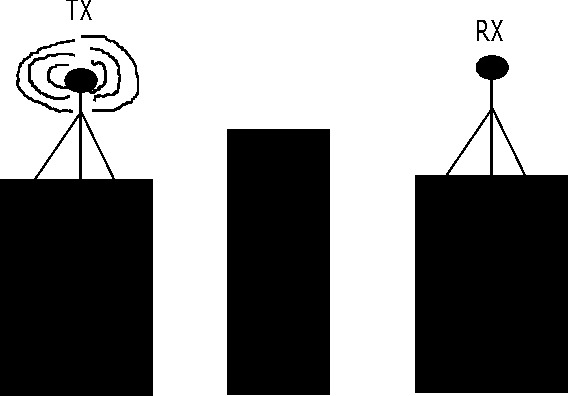
\includegraphics[width=0.35\textwidth]{los.pdf}
\caption{LOS illustration}
\label{LOS}
\end{figure}  


Where the counter-part is Non-Line-Of-Sight(NLOS)\citep{los}, which means that the path is interfered, which could be by a building standing in-between the transmitter antenna and the receiver antenna, where the two antennas cannot see each other, this is illustrated on the following Figure: 

\begin{figure}[H]
\centering
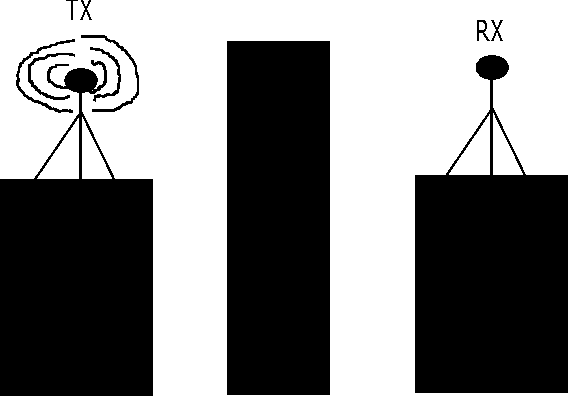
\includegraphics[width=0.35\textwidth]{nlos.pdf}
\caption{NLOS illustration}
\label{dijdkkfkfddd}
\end{figure} 

Another one is Near Line Of Sight(nLOS) \citep{los}, which means that the path is partially interfered,  which could be by a building. Which is illustrated on the following Figure:

\begin{figure}[H]
\centering
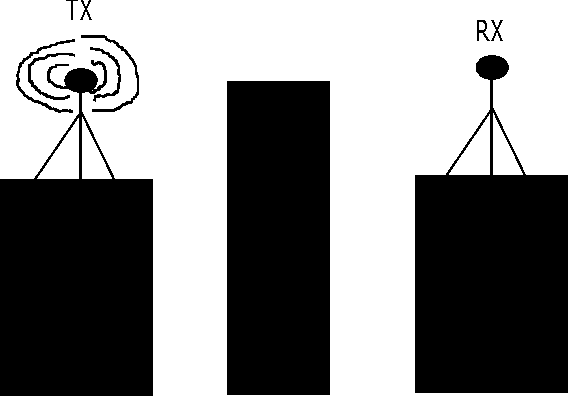
\includegraphics[width=0.35\textwidth]{nearlos.pdf}
\caption{nLOS illustration}
\label{nLOS}
\end{figure} 


The different line-of-sights, play a big factor when considering the Fresnel Zones which is further explained in worksheet Fresnel Zones, which also plays a big part in the received Power. As explained in the Fresnel Zone chapter there must be $60\%$ clearance in the first Fresnel zone, as the strongest signals are in the first Fresnel zone ,this could be a problem if there is too much NLOS, as the antennas would need to be risen higher.       







%interpolation 

%1M - rg223/u  22.41/100  = 0.224dB for 2.58 Ghz
%1M - rg223/u  12.7/100  =  0.127dB for 856  Mhz


%1.5M - SUCOFLEX_104 - attenuation factor_858  * 1.5 = 0.218 dB/M * 1.5M = 0.327dB  
%1.5M - SUCOFLEX_104 - attenuation factor_2.58 * 1.5 = 0.2386 dB/M * 1.5M = 0.579dB 

%2.20M - SUCOFLEX_104 - attenuation factor_858  * 2.20 = 0.218 dB/M  * 2.20M = 0.480dB
%2.20M - SUCOFLEX_104 - attenuation factor_2.58 * 2.20 = 0.2386 dB/M * 2.20M = 0.850dB




%If there is \textbf{NLOS}, shadowing must also then be considered as a part of the Link budget.
%\\
%\\
%Another thing to consider when, expecting the Power received is the Fresnel Zone which is further explained in Chapter \ref{fres_zone}    



\chapter{Far field and near field}
The fields surrounding the antenna, can be subdivided into two regions, far field and near field. A graphical illustration of the far field and near field \citep{farnear_field1}\citep{farnear_field2} can be seen on the following Figure:

\begin{figure}[H]
\centering
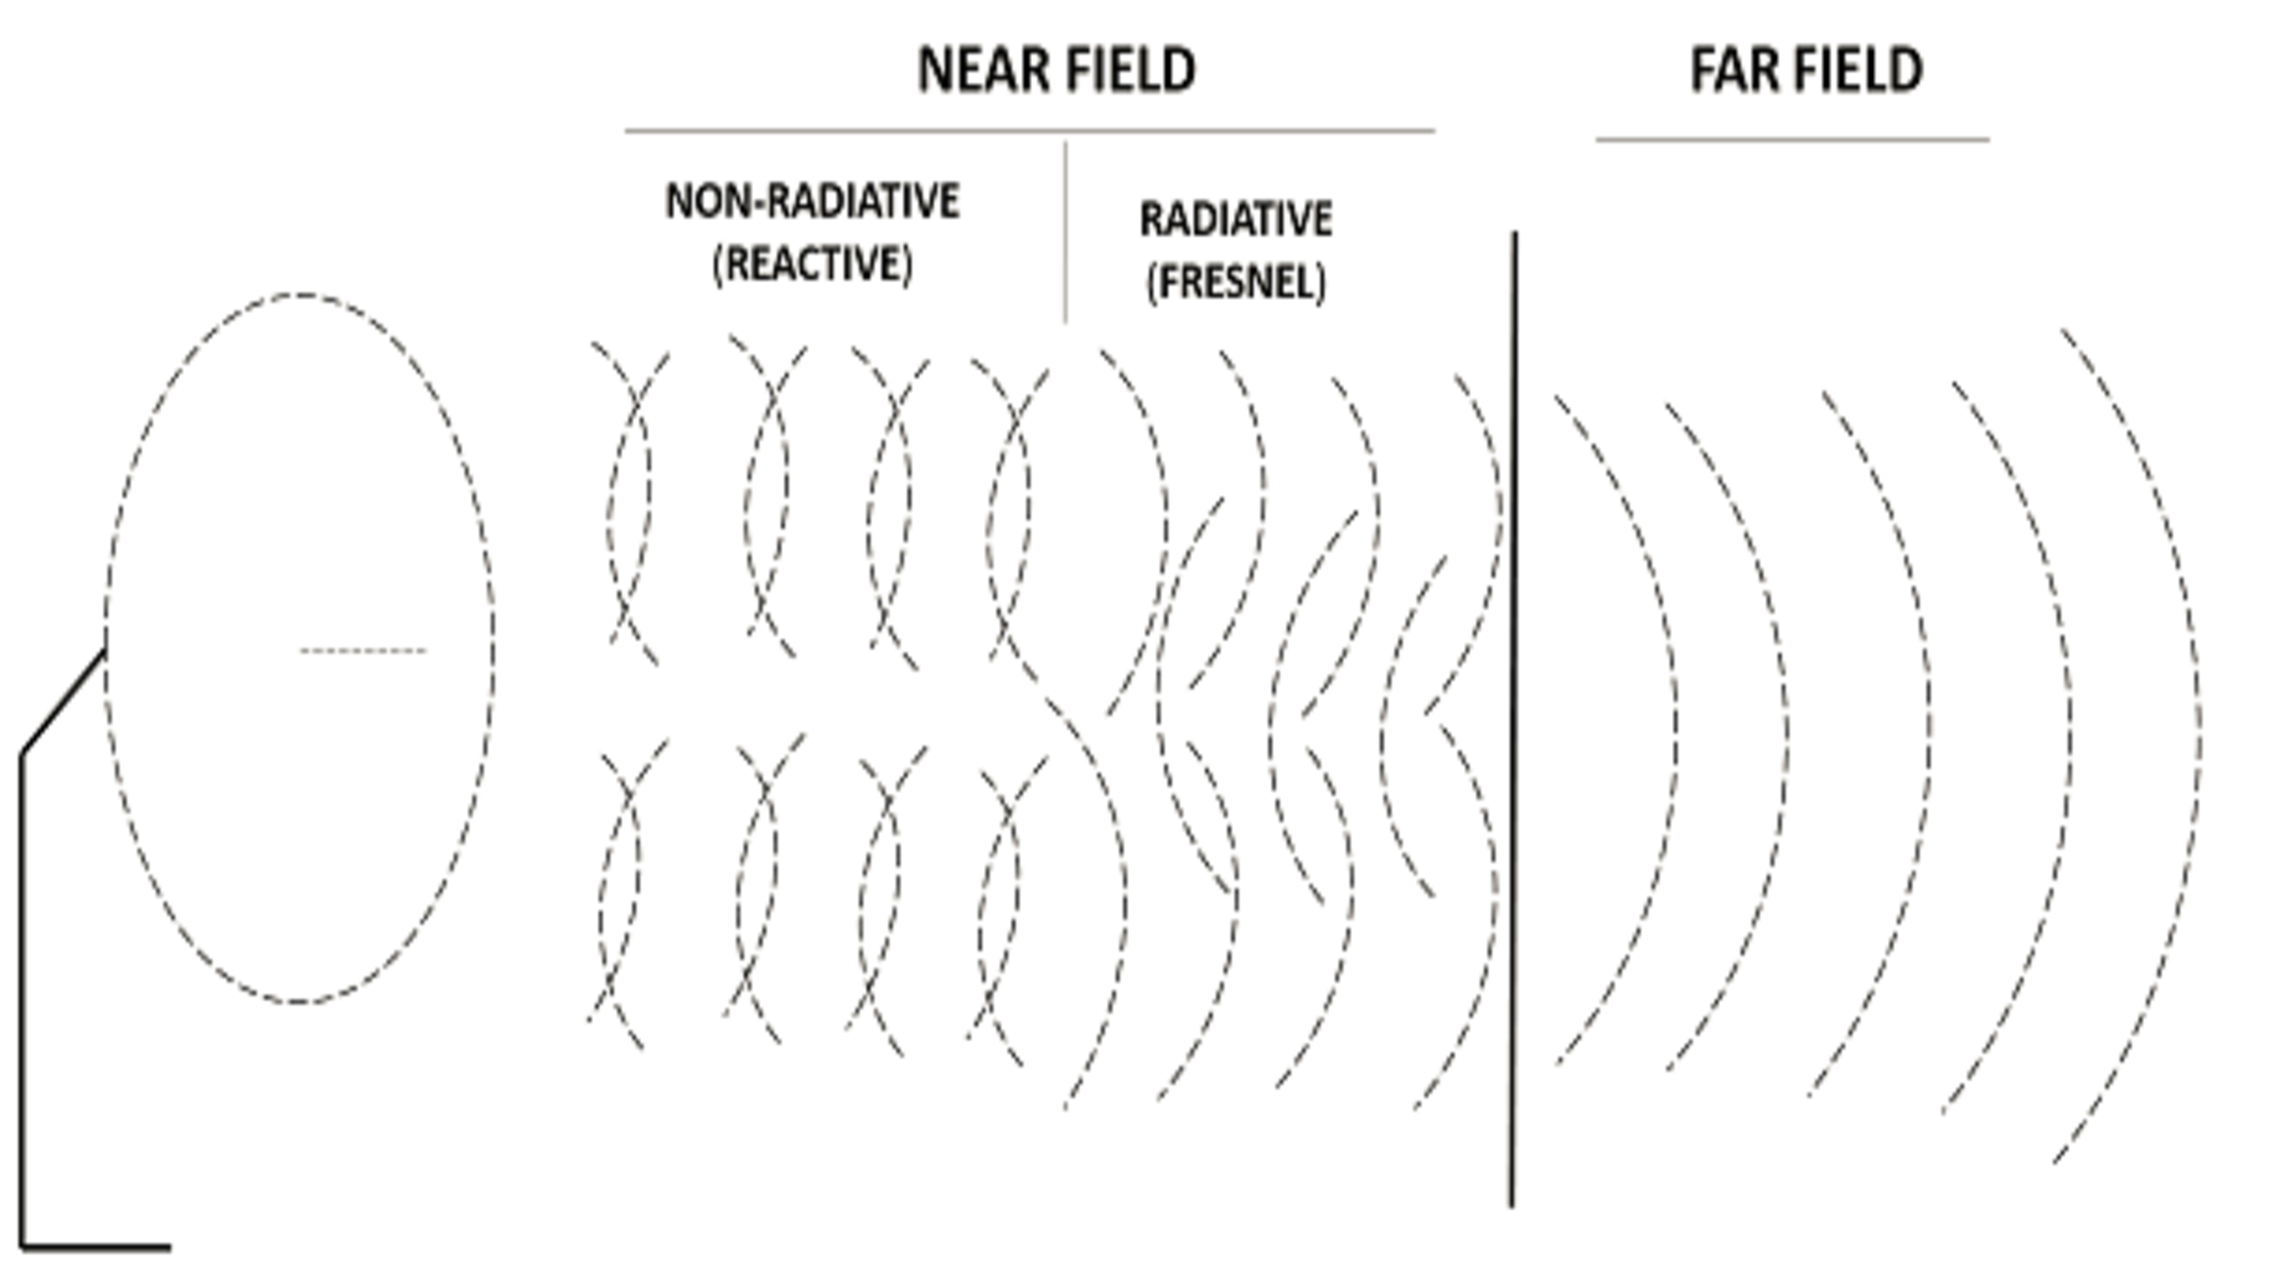
\includegraphics[width=0.6\textwidth]{nearfield_farfield.pdf}
\caption{Illustration of near field and far field \citep{farnear_field}}
\label{para_wave}
\end{figure}



\subsection{Far field region}

The far field region is the region that is furthest from the antenna. In this region the radiation pattern does not change shape with distance, and it is the region that it is desired to be in when measuring the power received. The far field region $R$ is given by the following formula:

\begin{equation}
R > \frac{2 \cdot D^{2}}{\lambda}
\label{far_field_eq1}
\end{equation}

\begin{where}
\va{$D$}{Is the maximum dimension of the antenna}{m}
\va{$\lambda$}{Wavelength}{m}
\end{where}

The far field region $R$ provides the limit between far field and near field. The far field region must also satisfy the following two equations:

\begin{equation}
R \gg D
\label{far_eq2}
\end{equation}

And

\begin{equation}
R \gg \lambda
\label{far_eq_3}
\end{equation}

The first two equations given in \ref{far_field_eq1} and \ref{far_eq2} ensure that the power radiated in a given direction from different parts of the antenna are approximately parallel. This helps to ensure that waves in the far field behave like plane waves. Plane waves only radiate towards the forward direction, and are in parallel. %This is illustrated on the following Figure:

%\begin{figure}[H]
%\centering
%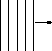
\includegraphics[width=0.2\textwidth]{para_wave.pdf}
%\caption{Illustration of Plane waves}
%\label{para_wave}
%\end{figure}

The third equation given in \ref{far_eq_3} makes sure that the reactive near fields are gone. The reactive near field is the region surrounding the antenna where the reactive field(standing waves or stored energy) are dominant. In a reactive field two oppositely waves are travelling, which are non-radiative, they do not radiate power, they store the energy. This means that the receiver antenna will not receive power in the near field, as it does not radiate. %So the receiver antenna will not receive these standing waves, as a part of the power radiated, in the far field. 
The much larger sign $\gg$ stands for 10 times larger. 
%The problem with the reactive field is that the receiving and the transmitting antenna may interact with each other 




%%http://my.ece.msstate.edu/faculty/donohoe/ece3323antennas.pdf
%%http://www.antenna-theory.com/basics/fieldRegions.php
%% https://www.tutorialspoint.com/antenna_theory/antenna_theory_near_and_far_fields.htm

%Reactive Near fields are unwanted as they radiate back and forward  




%The Far field region starts approximately two wave lengths from the antenna and extends outwards. 


%In this region the radiation pattern does not change with the shape of the distance  


\subsection{Near field region}

In the near field there are two regions the non-radiative(Reactive) and radiative(Fresnel) regions. The boundary for the non-radiative(Reactive) is given in the following Equation:

\begin{equation}
R < 0.62 \cdot \sqrt{\frac{D^{3}}{\lambda}}
\label{near_field_eq}
\end{equation}


While the radiative(Fresnel) region is the region between the near and far fields. In this region unlike for the far field region the shape of the radiation pattern may vary considerably with distance. The radiative(Fresnel) region is given by the following Equation:


\begin{equation}
0.62 \cdot \sqrt{\frac{D^{3}}{\lambda}} < R < \frac{2 \cdot D^{2}}{\lambda}
\label{far_field_eq1_2}
\end{equation}


The above can be summarized in the following Figure:

\begin{figure}[H]
\centering
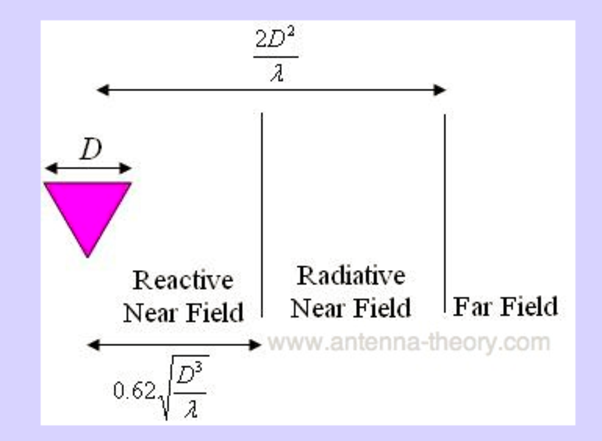
\includegraphics[width=0.5\textwidth]{nearfar_field_eq_ill.pdf}
\caption{Illustration of Near field and Far field \citep{farnear_field1}}
\label{nearfarf_eq_ill}
\end{figure}


\subsection{Far field Near field calculation}

\subsubsection{Patch 858Mhz}

In order to calculate if the measurements are done in the far field, the maximum dimension of a given antenna must be known. The maximum dimension $D$ is 0.105m, this given for the patch antenna of 858MHz. Then in terms of being in the Far field:

\begin{equation}
R > \frac{2 \cdot D^{2}}{\lambda}
\label{far_field_eq1_3}
\end{equation}



The wave length $\lambda$ for 868Mhz is given as:

\begin{equation}
\lambda = \frac{3E8 ms^{-1}}{0.868 Ghz} = 0.3453m
\end{equation}

Then:

\begin{equation}
R> \frac{2 \cdot (0.105m)^{2}}{0.3453m} = 0.0639 m 
\end{equation} 

While the minimum R is 1m, as the minimum distance between the transmitter and receiver antenna is 1 m. And as it can be seen, the first far field equation \ref{far_field_eq1_3} is fulfilled. 

The two other far field equations \ref{far_eq2} and \ref{far_eq_3}, the first one being:

\begin{equation}
1m \gg 0.105m
\end{equation}

Which is on the limit, to  being in the far field. While the third one given in \ref{far_eq_3}:

\begin{equation}
1m \gg 0.3453m
\end{equation}

This is not fulfilled, and therefore it is not in the far field the equation given in \ref{near_field_eq} is used.
\newpage

\subsubsection{Patch 2.58Ghz}

The dimension $D$ is 0.037m. The wave length $\lambda$ for 2.58GHz is given as:

\begin{equation}
\lambda = \frac{3E8 ms^{-1}}{2.58 GHz} = 0.1161m
\end{equation}

Then, for 1m:

\begin{equation}
1m > \frac{2 \cdot (0.037m)^{2}}{0.1161m} = 0.0235m
\end{equation} 

Again the first equation is fulfilled. While the second:

\begin{equation}
1m \gg 0.037m
\end{equation}

As it can be seen is fulfilled. While the third one:

\begin{equation}
1m \gg 0.1161m
\end{equation}



 





%\chapter{Small Scale Fading}

Small scale fading refers to small changes occurring both in the amplitude and phase over small distances, distances as small as half a wavelength. This means that the phase and amplitude keep changing, over small distances. The change in the amplitude and phase, is caused by multipath propagation and the Doppler shift.  
\\
\\
Multipath propagation is a result of reflecting objects and scatters in the propagation path.  
The received signal is the sum of all the signals arrived in different paths. Constructive summation of signals will cause an increase in the signal, while an de-constructive summation of the signals will cause an reduction of the signal, this all depending on how the phases of the signals add together. Deep fading may occur, which is a big loss of signal, where it could be that the two signals are out of phase. As the signals reflect and have an an direct way, this means that the signals have different lengths to arrive to the receiver, this causes the receiver to see multiple copies of the signal at different times of arrival.  


\subsection{Rayleigh Fading}
%Rayleigh fading does not consider the direct ray, which means that it only takes into account the reflection.
The Rayleigh distribution is good to use as a model for the channel propagation, when there is no strong line of sight path from the transmitter to the receiver. This could be when there is NLOS, where the transmitter is hidden behind a big building, where the transmitter cannot see the receiver, this will give a weaker line of sight signal.

\subsection{Rician Fading}
Rician fading distribution is used as a model for the channel propagation, when the direct line of sight is dominant, and there a few, reflected signals. 

%takes into account the LOS component to the  Rayleigh model, so it takes into account both the direct and the reflected signal. Rician fading is used when there is dominant non-stationary signal that is dominant. 




%%http://rfmw.em.keysight.com/wireless/helpfiles/n5106a/about_fading.htm

%%http://www.keysight.com/upload/cmc_upload/All/07-24-03-Fading-Schmitz_1mb-notes.pdf?&cc=DK&lc=dan

%%http://www.eee.hku.hk/~sdma/elec6040_2008/Part%204-Communications%20over%20wireless%20channels.pdf

%%http://www.iitg.ernet.in/scifac/qip/public_html/cd_cell/chapters/a_mitra_mobile_communication/chapter5.pdf

%%https://books.google.dk/books?id=OL7aBwAAQBAJ&pg=PA161&lpg=PA161&dq=small+scale+fading+rician&source=bl&ots=KPxUNkwLP0&sig=yQ20RMl17oV3mjrjbi30RWP94n8&hl=da&sa=X&ved=0ahUKEwjAhfKorI_QAhXCjCwKHbmXAtw4ChDoAQhGMAU#v=onepage&q=small%20scale%20fading%20rician&f=false

%%http://www.ee.fju.edu.tw/pages/032_faculty/sclin/lecture/wireless_comm/ch5.pdf

%%http://www.slideshare.net/nagasirisha756/3-thewirelesschannel2

%%http://www.planetanalog.com/document.asp?doc_id=527327
\cleardoublepage


%% problemanalysen %%
\pagenumbering{arabic} %use arabic page numbering in the mainmatter
\fancyfoot[RO,LE]{\thepage \text{ of} \pageref{LastPage}}
\fancyfoot[LO,RE]{16gr651}
\fancyhead[RE,LO]{}
\fancyhead[RO,LE]{\small\nouppercase\leftmark} %even page - chapter title



%\fancyhead[RO,LE]{\includegraphics[height=16pt]{logo_only.pdf}}


\pagestyle{fancy}
\makeatletter




%% literaturliste og bilag %%
\bookmarksetup{startatroot}% this is it
\addtocontents{toc}{\bigskip}% perhaps as well
\bibliography{setup/mybib}
\label{bib:mybiblio}
 
% \newpage
 \fancyhead[RO]{\small Appendix \nouppercase\rightmark} %even page - chapter title
 \fancyhead[LE]{\small Appendix \nouppercase\rightmark} %uneven page - section title
\fancyhead[RE,LO]{}
 \titleformat{\section}[hang]{\Large\bfseries}{\thesection\hsp\textcolor{black}{|}\hsp}{0pt}{\Large\bfseries}

 \renewcommand{\thesection}{\Alph{section}}
 \setcounter{section}{0}




%\chapter*{Appendix}
 %\addcontentsline{toc}{chapter}{Appendix}
 %\addtocounter{chapter}{1}


\end{document}